\newpage
\section{Bateau}

\begin{figure}[h]
    \centering
    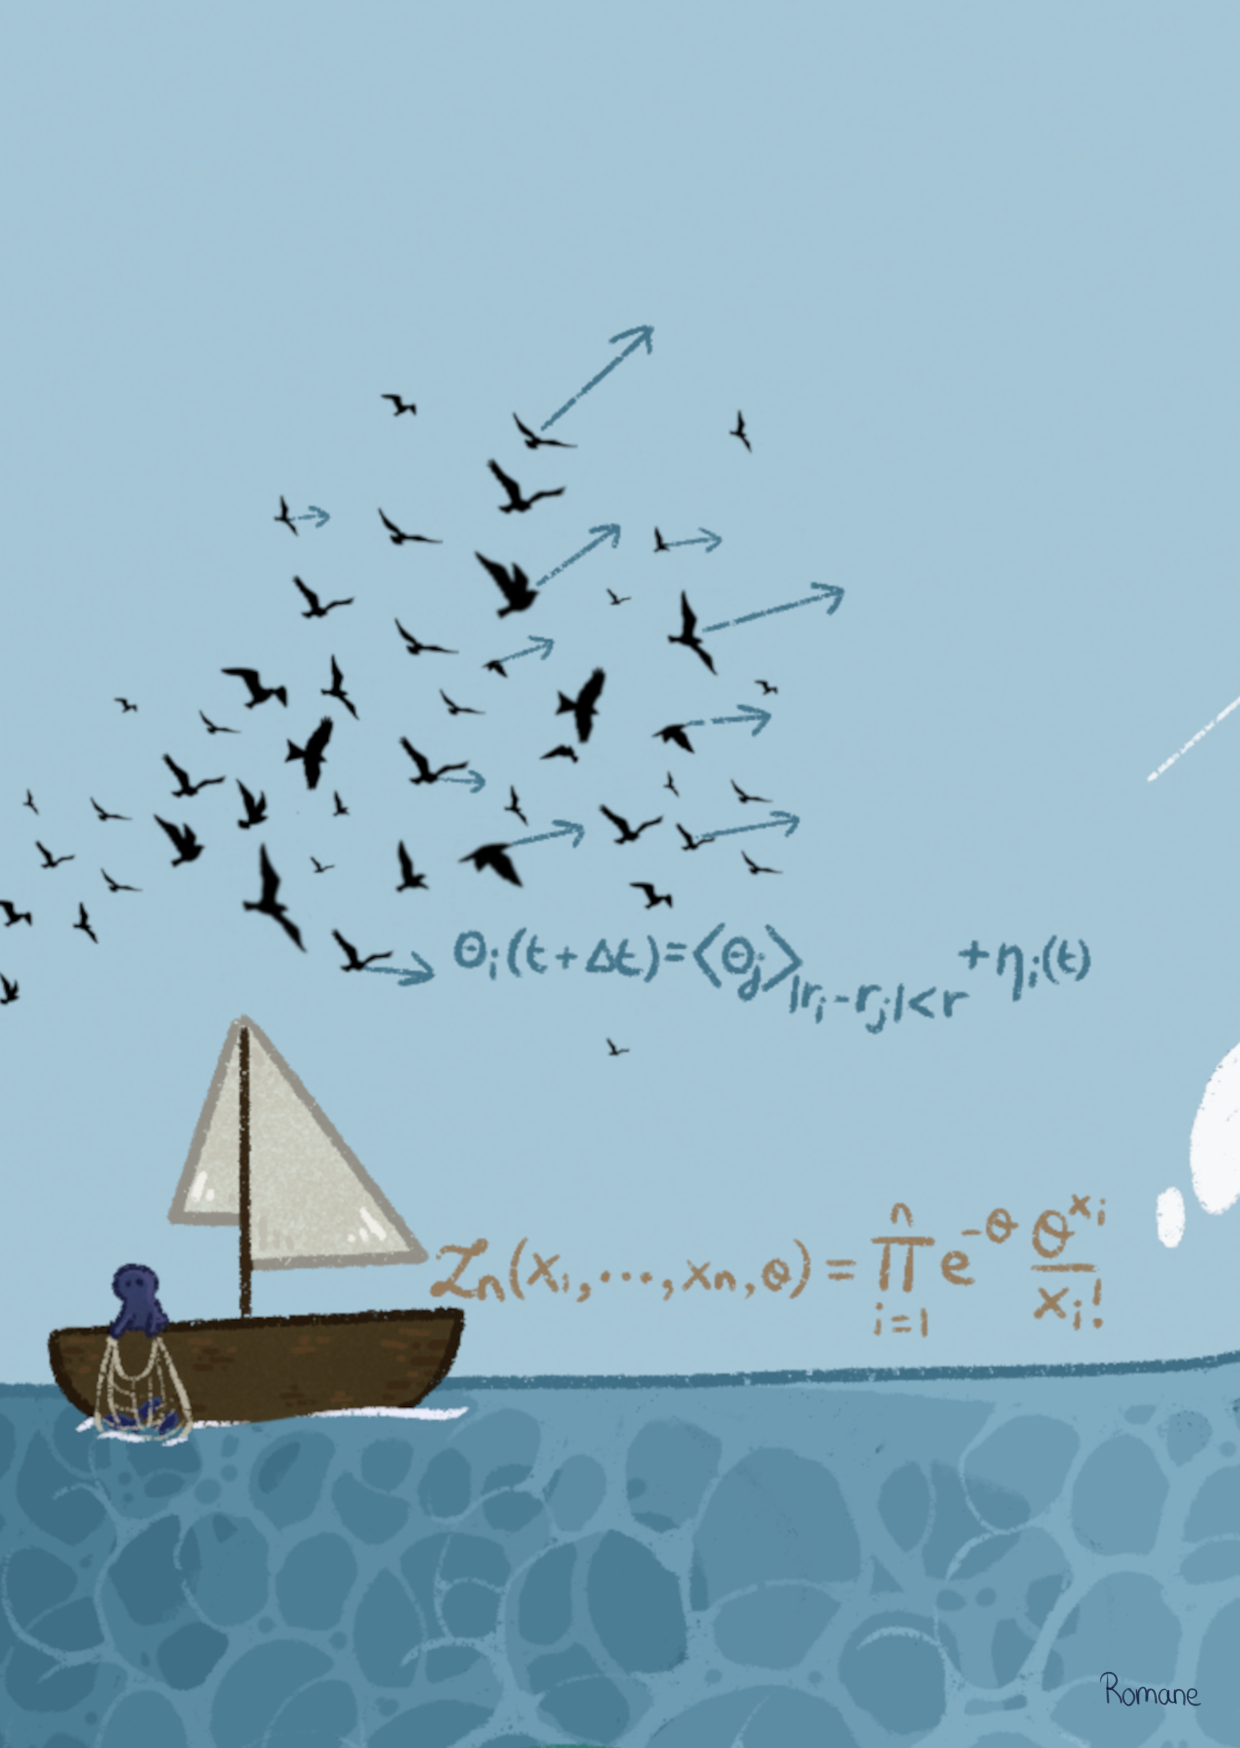
\includegraphics[height=0.5\textheight]{Cartes_postales/carte01-bateau.png}\label{fig:c1}
    \caption{Carte postale: Bateau}
\end{figure}

Sais-tu qu'on peut estimer le nombre de truites en mer? Pour cela, on utilise une méthode mathématique appelée capture-recapture. On commence par capturer des truites, on les marque et puis, on les relâche. Après un certain temps, on capture à nouveau des truites, c'est la recapture. On suppose que la proportion de truites marquées dans notre recapture parmi toutes les truites de notre recapture est la même proportion que celle de toutes les truites marquées parmi toutes les truites:

\begin{figure}[h]
    \centering
    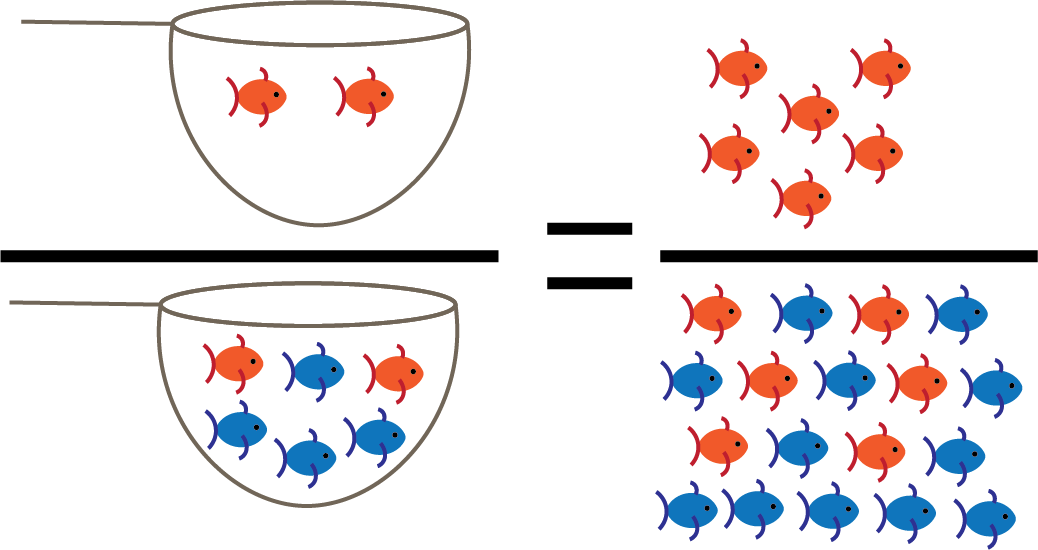
\includegraphics[height=0.1\textheight]{Images/poissons_v2.png}\label{fig:c1_poissons}
    \caption{Illustration de la formule}
\end{figure}

On peut en déduire une estimation du nombre total de truites en mer avec un produit en croix. En pratique, on utilise des méthodes plus poussées, toujours basées sur cette idée, car on rencontre beaucoup de problèmes liés au fait qu'on estime des populations d'êtres vivant, contrairement aux cours de maths où on compte des billes dans un sac. Voici quelques problèmes qu'on peut rencontrer: les marquages peuvent s'effacer, le nombre total de truites change, la population se dépace ailleurs. C'est pour ça qu'il y a beaucoup de recherches mathématique sur ces sujets.